\section{ساختاربندی مطلب}
\begin{frame}{انتخاب محیط کلی سند}
\begin{itemize}\itemr
\item[-] 
در ابتدایی‌ترین خط یک فایل 
\lr{tex}
باید نوع آن را مشخص کرد،

\item[-]
این کار با دستور 
\lr{\texttt{\textbackslash documentclass\{class\}}}
انجام می‌شود.

\item[-]
محیط‌های مختلفی از جمله
\lr{\texttt{article}}،
\lr{\texttt{report}}،
\lr{\texttt{book}} و
\lr{\texttt{letter}}
و موارد زیاد دیگری‌ست که لیست بلندی از آن‌ها در 
\url{https://ctan.org/topic/class}
موجود است.
\end{itemize}
\end{frame}

\begin{frame}{اضافه کردن زبان فارسی}
\begin{itemize}\itemr
\item[-] 
سپس باید پشتیبان زبان فارسی را به لاتک اضافه کرد،

\item[-]
این کار با دستور 
\lr{\texttt{\textbackslash usepackage\{xepersian\}}}
انجام می‌شود.

\item[-]
این بسته نیازمند یک فونت فارسی هم هست که با دستور 
\lr{\texttt{\textbackslash settexfont\{FONT\}}}
انجام می‌شود.
\end{itemize}
\end{frame}

\begin{frame}{ساختاربندی سند}\label{parts-chapters}
\begin{itemize}\itemr
\item[-]
تگ‌های زیر برای قسمت‌بندی و تعیین ساختار سند استفاده می‌شوند

\begin{center}
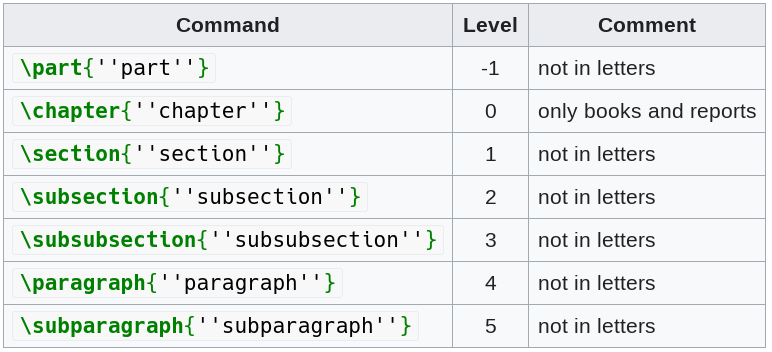
\includegraphics[width=0.63\textwidth, height=0.53\textheight]{docs/images/sections} 
\end{center}
\end{itemize}
\end{frame}

\begin{frame}{نمونه‌های تگ‌های ساختاربندی}
\begin{itemize}\itemr
\item[]
\begin{center}
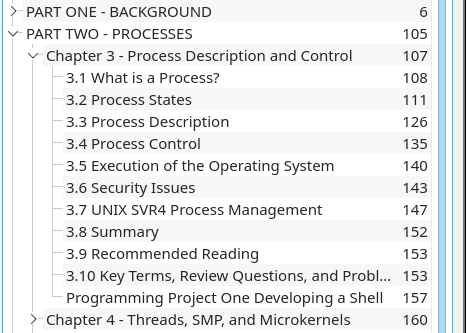
\includegraphics[width=0.5\textwidth, height=0.6\textheight]{docs/images/secexample}
\end{center}
\end{itemize}
\end{frame}

\begin{frame}[fragile]{نمونه کد}
\begin{latin}
\begin{lstlisting}[keywords={part, chapter, section, subsection}, keywordstyle=\color{Mulberry}\textbf]
\begin{document}
\chapter{History}

\section{Creation}

\subsection{Who}
Donald Knuth

\subsection{When}
1978; 45 years ago
\end{document}
\end{lstlisting}
\end{latin}
\end{frame}

\begin{frame}{خروجی}
\begin{center}
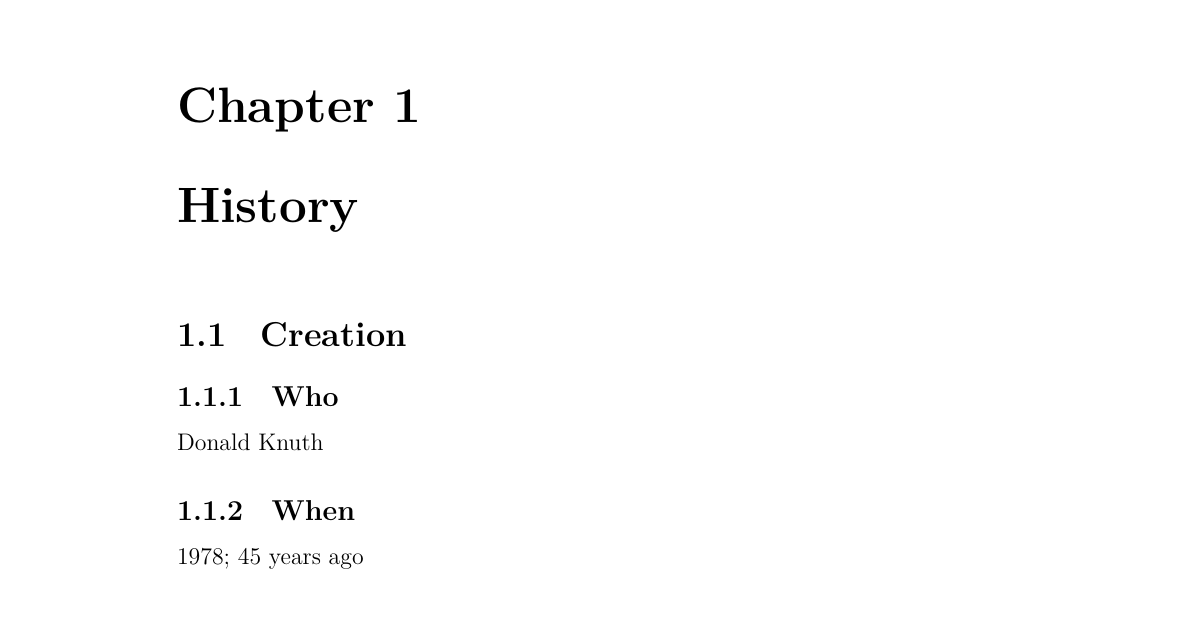
\includegraphics[width=0.7\textwidth, height=0.6\textheight]{docs/images/chsec}
\end{center}
\end{frame}

\begin{frame}{خروجی}
\begin{center}
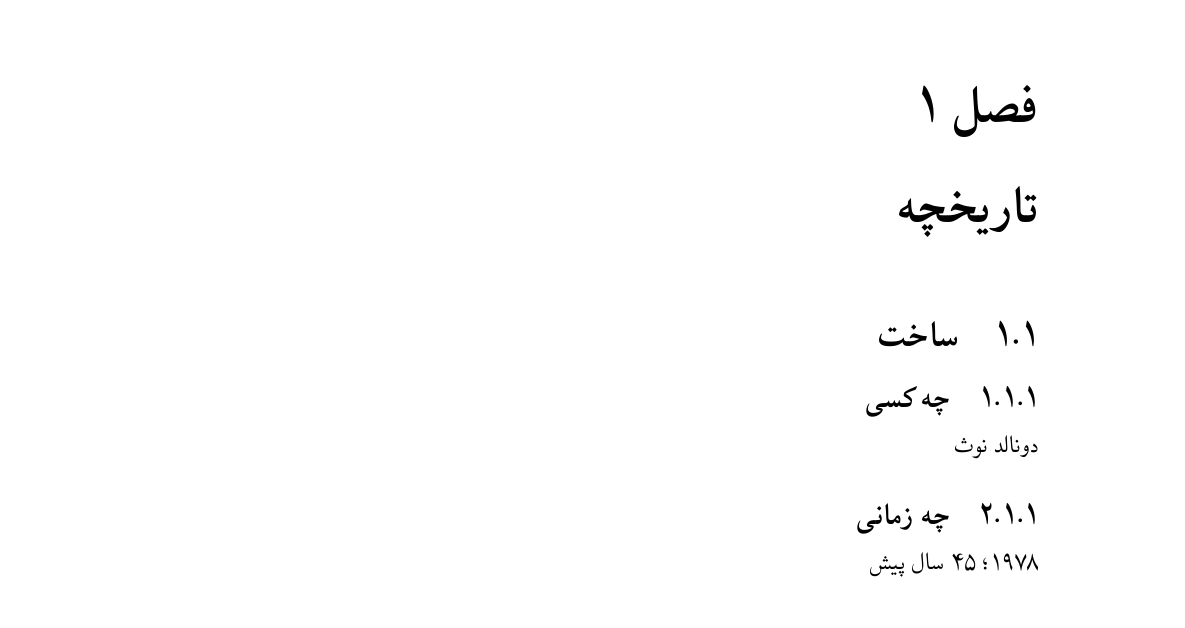
\includegraphics[width=0.7\textwidth, height=0.6\textheight]{docs/images/chsec-fa}
\end{center}
\end{frame}